\documentclass[12pt,letterpaper]{article}
\usepackage{amsmath} % just math
\usepackage{amssymb} % allow blackboard bold (aka N,R,Q sets)
\usepackage{ulem}
\usepackage{graphicx}
\usepackage{float}
\linespread{1.6}  % double spaces lines
\usepackage[left=1in,top=1in,right=1in,bottom=1in,nohead]{geometry}
\usepackage{caption}
\usepackage{subcaption}
\usepackage{floatrow}
\usepackage{blindtext}


\begin{document}
\setcounter{subsection}{1} 
\begin{flushright}
\end{flushright}
\begin{flushleft}
\textbf{Eric Zounes, Ian Fridge} \\
\today \\ 
CS434: Assignment 2 
\end{flushleft}
\section[1.]{Implementation Assignment} 
In this assignment we implement a top-down greedy induction algorithm for learning decision trees. In this example we have a data set containing a set of features which describe a monk. There are 6 features provided below: \\
$ x_{1}: $head\_shape$	\in round, square, octagon$ \\
$ x_{2}: $body\_shape$ 	\in round, square, octagon$ \\
$ x_{3}: $is\_smiling$	\in yes, no$ \\
$ x_{4}: $holding$	\in sword, balloon, flag$ \\
$ x_{5}: $jacket\_color$	\in red, yellow, green, blue$ \\
$ x_{6}: $has\_tie$	\in round, square, octagon$ \\

The class label is a concept defined by the following rule: \\
$($head\_shape$ = $body\_shape$) or ($jacket\_color$ = $red$)$ \\
If $x_{2} = x_{1}$ or $x_{5} = 1, y = 1$ \\
As mentioned, please learn 1. a decision stump; and 2. a depth-2 decision tree from the training data. Include: \\
\begin{enumerate} 
	\item[1.] Both the learned stump and the depth-2-decision tree. To help grading easier, please provide for each selected test its information gain.  
	\item[2.] The training and testing error rate of the learned stump and depth-2 decision tree. 
\end{enumerate} 
Finally, please answer the following questions: 
\begin{enumerate} 
	\item Given the formula for generating the class label, please provide (as compact as possible) decision tree that will correctly classify all training examples. 
	\item Do you expect the top-down greedy induction algorithm to learn this optimal tree?


\begin{table*}[htbp]
 \centering
\begin{minipage}[b]{5in}
 \centering
    \begin{tabular}[H]{ | l | l |}
    \hline
    Tree Depth & Error Rate \\ \hline
    1          & 0.250 \\ 
    2          & 0.301 \\
    3          & 0.317 \\
    \hline
    \end{tabular}
    \caption{Error Rate on Testing Data}
    \label{labelname 1}
\end{minipage}

\begin{minipage}[b]{5in}
 \centering
    \begin{tabular}[H]{ | l | l |}
    \hline
    Tree Depth & Error Rate \\ \hline
    1          & 0.266 \\ 
    2          & 0.287 \\
    3          & 0.255 \\
    \hline
    \end{tabular}
    \caption{Error Rate on Training Data}
    \label{labelname 2}
\end{minipage}
\end{table}

\begin{figure}[h!]
  \centering
      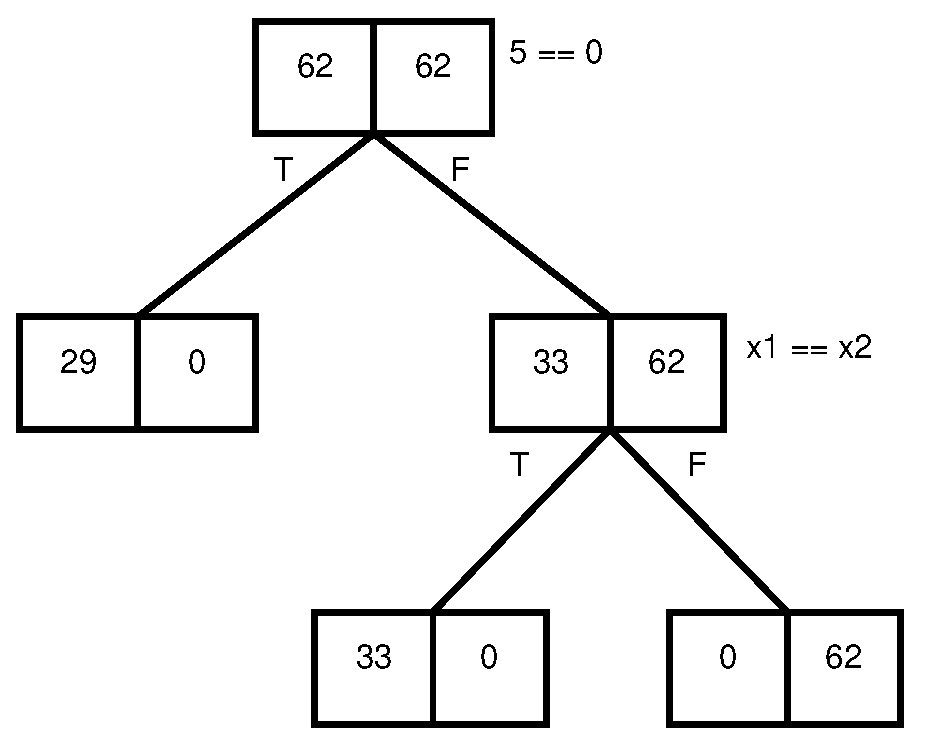
\includegraphics[width=4in]{BPerfect.eps}
  \caption{Depth 2 Learned Decision Tree}
\end{figure}

\begin{figure}[h!]
  \centering
      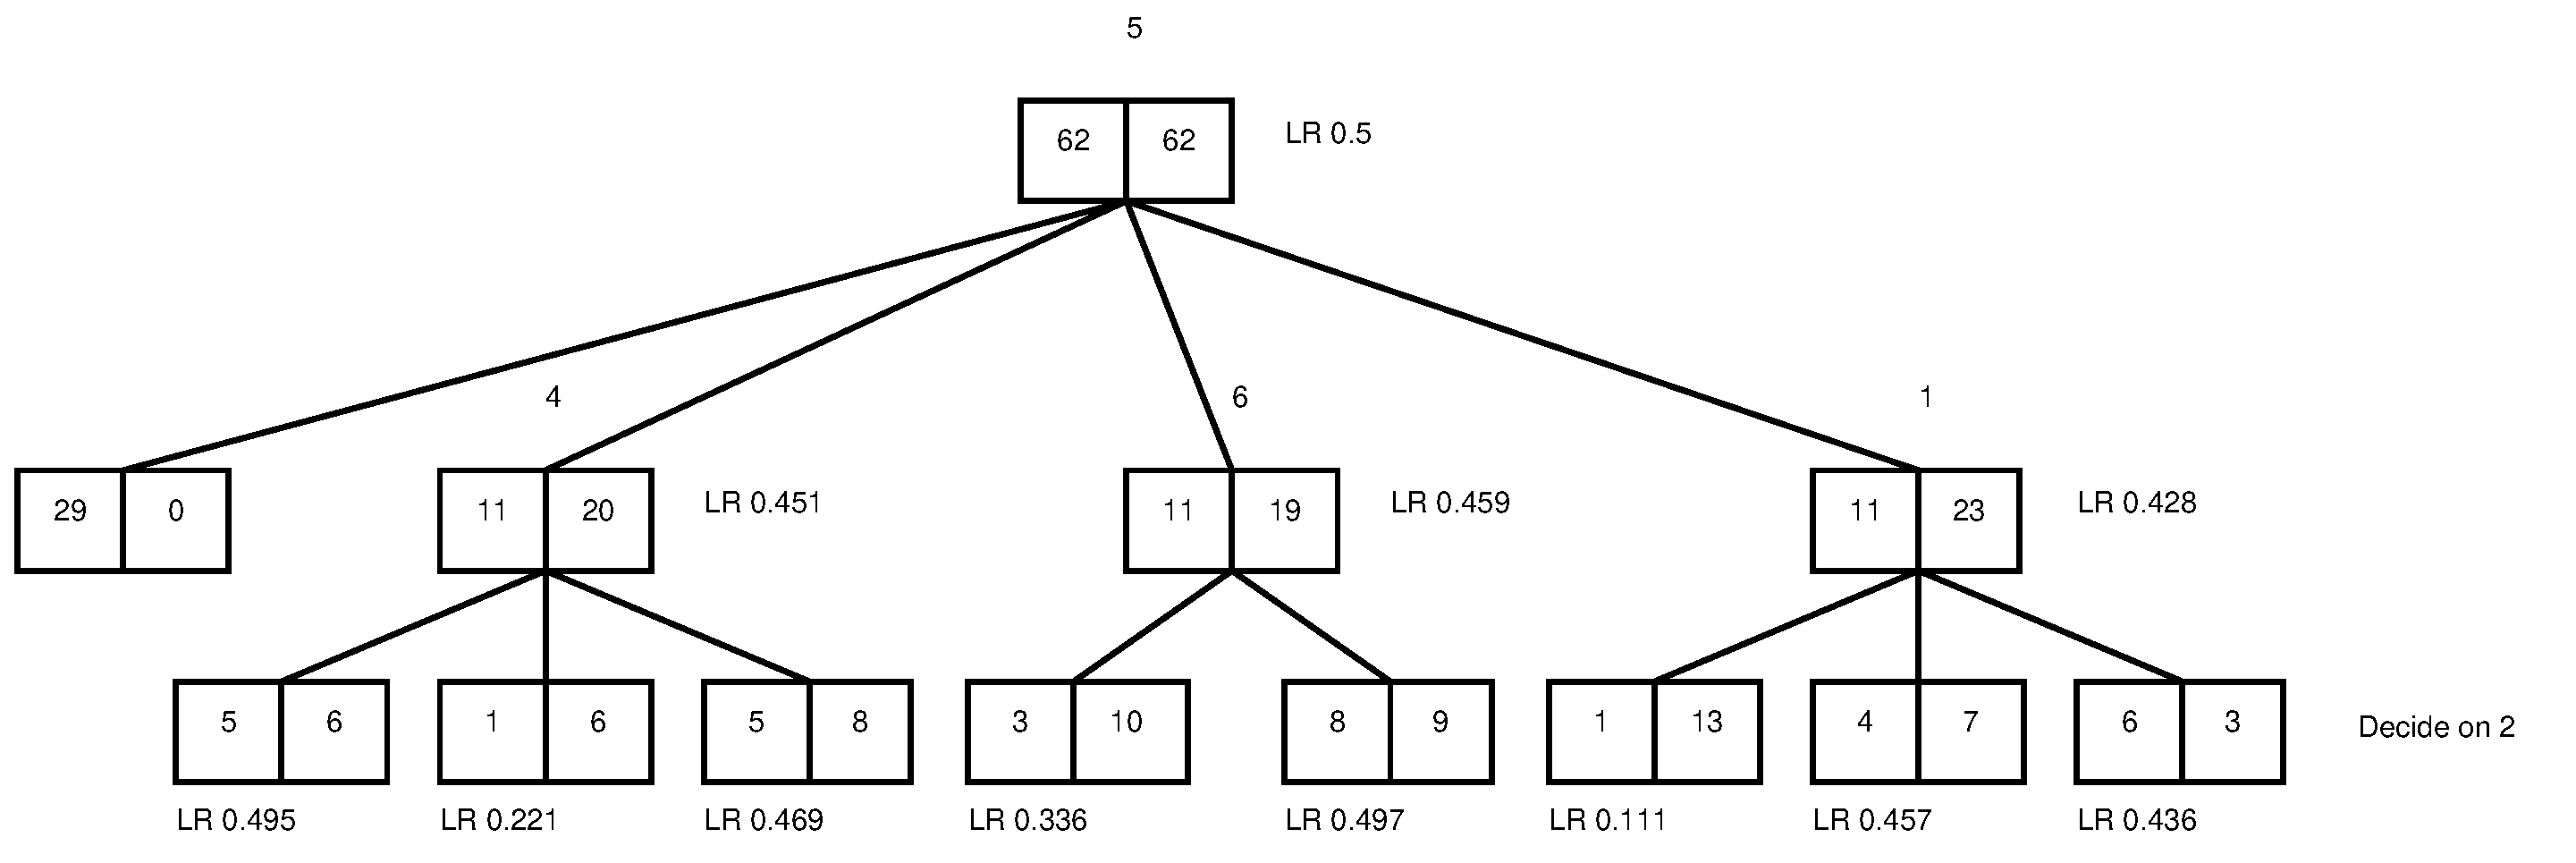
\includegraphics[width=7in]{D2.eps}
  \caption{Depth 2 Learned Decision Tree}
\end{figure}
\end{enumerate}

\subsection{Class Label Graph}
The ideal graph would be to classify based on each of the clauses of the rule.  The best possible algorithm that our algorithm could have learned would be to split upon the value of $x5$ which gives you one leaf node and then split the remaining children on $x1$ and $x2$ in either order.  When our algorithm was used to create a depth 3 tree we found that the algorithm chose $x2$ for one of the siblings after the first level of the tree.  All of this node's children choose 1 as the classifying feature to split on.  This tree would then cover all of the rules to contain all of the true cases in leaf nodes 
 
\subsection{Ideal Trees and the Top-down Greedy Induction Algorithm}
Generally the greedy induction algorithm will not create optimal decision trees.  While it can make locally optimal decisions for each node it does not neccesarily make decisions which are globally optimal.  Many of the branches in the decision tree are not relevant to the classifying rule.  When looking at a depth 2 tree created by the algorithm we see that it does make some correct decisions however it chooses several other values to partition upon which were not useful for finding the rule.  

\subsection{Testing and Training Error}
The difference between the testing and training error would suggest that there were signs of overtraining as the the error rate seemed to increase with after the first 
 
\section[2.]{Individual Assignment} 
\begin{enumerate} 
	\item We have two identical bags. Bag A contains 4 red marbles and 6 black marbles. Bag B contains 6 red marbles and 6 black marbles. Now we randomly chose a bag and drew a marble from the chosen bag and it turns out to be black. What is the probability that the chosen bag is bag A? \\
	To solve this problem we can use the Bayes rule. \\
	$ P(A|B) = \frac{P(B|A)P(A)}{P(B|A)P(A) + P(B|~A)P(~A)}$ \\
	Bag: $\in {A,B}$ \\
	Marble: $\in {red,black}$ \\
	We can define event: \\
	$A =$ Obtained black marble \\
	$B =$ Obtained bag A \\
	$P(B) = .5$, $P(A) = .6$ \\
	$P(A|B) = \frac{.3*.5}{.3*.5 + .5*.5*.5} = 55.45\%$ \\
	\item Suppose we have class variable y and three attributes $x_{1}, x_{2}, x_{3}$ and we wish to calculate $P(y = 1 | x_{1} = u_{1}, x_{2} = u_{2}, x_{3} = u_{3})$, and we have no conditional independence information. \\
	\begin{enumerate}
		\item Which of the following sets of probabilities are sufficient for calculation? \\
		\begin{enumerate} 
			\item $P(y = 1); P(x_{1} = u_{1} | y = 1); P( x_{2} = u_{2} | y = 1); P(x_{3} = u_{3} | y = 1)$ \\
			\item $P(x_{1} = u_{1}, x_{2} = u_{2}, x_{3} = u_{3}); P(y = 1); P(x_{1} = u_{1}, x_{2} = u_{2}, x_{3} = u_{3} | y = 1)$ \\
			\item $P(y = 1); P(y = 1| x_{1} = u_{1}); p(y = 1 | x_{2} = u_{2}); P(y = 1 | x_{3} = u_{3})$ \\
		\end{enumerate} 
		The 2nd example is sufficient because the probability of each feature must be taken in to account since we have no information about independence.\\
		\item Now suppose we know that the variables $x_{1},x_{2},x_{3}$ are conditionally independent given the class variable Y. Which of the above 3 sets are sufficient now? \\
		The 1st one is sufficient since we can calculate the P of each feature independently given the prior.\\
	\end{enumerate} 
	\item (Naive Bayes Classifier) We will use the following training set to build a Naive Bayes classifier. A, B, and C are three binary attributes and Y is the target class label. \\[10mm]
	\centering
	\begin{tabular}{| l | l | l | l |} 
	\hline
	A & B & C & Y \\ \hline 
	0 & 1 & 1 & 0 \\ \hline
	1 & 1 & 1 & 0 \\ \hline
	0 & 0 & 0 & 0 \\ \hline
	1 & 1 & 0 & 1 \\ \hline
	0 & 1 & 0 & 1 \\ \hline
	1 & 0 & 1 & 1 \\ \hline 
	\end{tabular} \\[15mm]
	\begin{enumerate} 
		\item Based on the training data, calculate the prior distribution for Y:P(Y), with and without Laplace smoothing. \\
		$P(y = j) = \frac{1}{n} \sum_{i=1}^{n} I(y_{i} = j)$ \\
		There are 6 examples and a binary class. So, we can say: \\
		$\frac{1}{6} \sum_{i=1}^{6} I(y_{i} = 1)$ \\
		$\frac{3}{6} = .5$ \\
		With Laplace smoothing we obtain: \\
		$\frac{3+1}{6+2*1}i = .5$ at $ k = 1$ \\ 
		We are essentially adding two additional samples with each classifier to increase our resolution. \\ 
		\item Based on the training data, calculate the distributions $P(A|Y), P(B|Y)$ and $P(C|Y)$, with and without Laplace smoothing. \\
		Without Laplace smoothing we obtain: \\
		$P(A|Y) = \frac{2}{6} = .33$, $P(B|Y) = \frac{2}{6} = .33$, $P(C|Y) = \frac{1}{6} = .16$ \\
		With Laplace smoothing we obtain: \\
		$P(A|Y) = \frac{2+1}{6+2*1} = .375$, $P(B|Y) = \frac{2+1}{6+2*1} = .375$, $P(C|Y) = \frac{1+1}{6+2*1} = .25$ \\
		\item What prediction will the Naive Bayes classifier make for a new example $(A = 1, B = 0, C = 0)$, with and without Laplace smoothing? \\
		In order to test this new example we must find: \\
		$P(y = 1)*P(A = 1 | y = 1)*P(B = 0 | y = 1)*P(C = 0 | y = 1)$ \\
		and \\
		$P(y = 0)*P(A = 1 | y = 0)*P(B = 0 | y = 0)*P(C = 0 | y = 0)$ \\
		 $\frac{3}{6} * \frac{1}{3} * \frac{1}{6} * \frac{1}{3} = .00925$ \\
		 $\frac{3}{6} * \frac{1}{6} * \frac{1}{6} * \frac{1}{6} = .00231$ \\
		Thus, the new example is $\in y = 1$ \\
		With Laplace smoothing: \\
		 $\frac{3+1}{6 + 2*1} * \frac{1+1}{3 + 2*1} * \frac{1 + 1}{6 + 2*1} * \frac{1 + 1}{3 + 2*1} = .00200$ \\
		 $\frac{3+1}{6 + 2*1} * \frac{1+1}{6 + 2*1} * \frac{1 + 1}{6 + 2*1} * \frac{1 + 1}{6 + 2*1} = .00781$ \\
	\end{enumerate}
	\item Decision tree learning \\
	Given the following data set: \\[15mm]
	\begin{tabular}{c | c | c || c } 
	V & W & X & Y \\ \hline
	0 & 1 & 0 & 1 \\ \hline
	1 & 0 & 0 & 1 \\ \hline 
	1 & 1 & 0 & 0 \\ \hline 
	1 & 1 & 1 & 0 \\ \hline 
	\end{tabular} \\[15mm]
	The task is to build a decision tree for classifying Y. \\
	\begin{enumerate} 
		\item Compute the information gain of attributes X, V, and W respectively. \\
		$-\frac{2}{4}log_{2}\frac{2}{4} -  $
		\item Use information gain for selecting test and produce the full decision tree. \\

		\item Considering the following two strategies for avoid over-fitting. \\

		\begin{enumerate} 
			\item The first strategy stops growing the tree when the information gain of the best test is less than a given threshold $\epsilon$. \\
			\item The second strategy grows the full tree first and then prunes the tree bottom up: start from the lowest level of the tree and prune a sub-tree if the information gain of the test is less than a given threshold $\epsilon$. (Note that you should stop checking level $t$ if none of sub-trees at level $t+1$ satisfies the pruning criterion.i) \\
		Let $\epsilon$ be $0.001$ for both cases, write down the resulting tree for each strategy and compare their training errors. \\
		\end{enumerate} 	
		\item Discuss the advantages and disadvantages of the two strategies. \\
	\end{enumerate} 
	\item Show that logistic regression learns a linear decision boundary. \\
	Since $P(y = 1 | x) = \frac{1}{1 + e^{-w*x}} > P(y = 0 | x) = \frac{e^{-w*x}}{1 + e^{-w*x}}$ \\
	We know that: \\
	$log(\frac{P(y = 1 | x)}{P(y = 0 | x)} = w_{0} + w_{1}x_{1}) + \ldots + w_{m}x_{m}$ \\
	If we substitute in our equations for P we get: \\
	$log(\frac{1 + e^{-w*x}}{e^{-w*x}(1 + e^{-w*x}})) = log(e^{w*x}) = w*x$ \\
	Therefore, since the rate of change is constant and it's continuous, we can say that this equation for the decision boudary is linear. \\
\end{enumerate}
\end{document} 
